% !TeX root = ../SPL-Rules.tex
% !TeX spellcheck = en_US
\section{The Official RoboCup Competition Rules}
\label{sec:comRules}
This section contains rules that are not directly relevant for games and that may not apply at local opens.  However, these rules will be upheld at the yearly international RoboCup competition.

\subsection{Qualification Procedure and Code Usage}
\label{sec:qualification_procedure_codeuse}

The qualification procedure as well as the corresponding deadlines will be announced by the Technical Committee before qualification applications are accepted.

The RoboCup Standard Platform League offers unique possibilities to use code from other teams. In spirit of the RoboCup every team is generally allowed to use code from other teams to push the league further with their own research.
This use must be cited.
However, every participant of RoboCup \textbf{\textit{has a duty}} to contribute to the league.

To qualify, every team must make at least \textit{novel contribution} within their soccer software.
A team must have made at least one contribution within the last \NovelContributionTime.
Contributions outside of this period are no longer considered sufficiently novel and a team must make at least one \textit{new} contribution.
It is also \textit{mandatory} for a team to use their novel contribution in all competition games.
A novel contribution is:
\begin{itemize}
  \item Research publishable contribution to a \textit{game critical module}
  \item Complete replacement of a \textit{game critical module}, with original software. This may not necessarily be research publishable, but must be of equivalent scale and quality to research publishable work.
\end{itemize}

It is not a novel contribution to replace a module with code copied from another source, or to simply train a machine-learning model released by another team using new data.

As of the 2022 competition, the following are recognized as game critical modules:
Ball detection, Robot detection, Robot vision (not otherwise listed), Localization, Walk/Kick engine, Dynamic stabilization, Behavior Architecture, \& Distribution computation, Whistle detection.

As of the 2022 competition, the following are \textit{not} recognized as sufficiently game critical (even if the ability to play soccer depends on these):
Hand-written Soccer Behaviors, Natural Language detection, \& Robot and GC Communication.

In their qualification application, teams may petition the technical committee to recognize other novel contributions not listed here.
Additionally, a team that has participated at RoboCup for at least \NovelContributionTime consecutively may petition the technical committee to recognize contributions to non-game critical modules, such as developing infrastructure for the league\footnote{However, the technical committee should balance whether a team is continuing to use their own software in games.}.
A team may also petition for the technical committee to reconsider the list of game critical and non-game critical modules.
Successful petitions will be public ally announced to the league for transparency.
%For example, a team may petition and provide evidence that their work on the whistle detection is substantial and game critical, thus satisfying the requirements of a novel contribution.

If a team that is otherwise eligible for qualification cannot provide sufficient evidence of the required contributions by the deadline for applications, then that team may be qualified for RoboCup \textit{on probation}.
In this case, the team must provide evidence of the required contributions to become \textit{fully} qualified by the registration deadline of the RoboCup event.
If no suitable evidence is provided, the team's probationary qualification will lapse.

Every applicant must also bring a poster containing the team's contribution, focused on the current year, to the RoboCup event to share their contributions with the other teams.

Failure to meet any of these requirements will result in a qualification penalty for subsequent years.

\subsection{Game Structure}

The clock stops during stoppages of play (such as ready and set state after goals) from the knock-out competition onwards.  In round-robin pool play, a game may finish in a draw and there will be no penalty shoot-out, like in all other games (see Section~\ref{sec:penalty_shoot-out}).

\subsection{Champions Cup and Challenge Shield}
\label{sec:twoCompetitions}

To provide better matched games for teams of all abilities the RoboCup Standard Platform League shall be divided into two separate competitions: the Champions Cup for the strongest teams and the Challenge Shield for all other teams. Champions Cup and Challenge Shield teams compete separately in each tournament. Teams are promoted to (or relegated from) the Champions Cup during the tournament. 

There are 24 qualified teams. 12 teams are placed in the Champions Cup. 12 teams are placed in the Challenge Shield. Teams retain their placing in the Champions Cup or Challenge Shield between each year, unless otherwise promoted or relegated as described below.
All qualified teams are ranked using the Glicko system\footnote{\url{http://www.glicko.net/glicko/glicko.pdf}} based on all available results from previous official RoboCup tournaments. (New teams will be ranked equally below all previously competing teams. Teams that participated previously but did not participate in the previous year will be ranked above new teams but below teams that competed in the previous year.)

\subsubsection{Tournament Structure}
\emph{This structure may be revised by the TC/OC based on game scheduling constraints.}

The Champions Cup and Challenge Shield follow the same structure as independent competitions. They are referred to as ``divisions'' below for clarity.

Each division will have a round-robin stage, and a knockout competition. The round-robin stage consists of 2 groups of 6 teams. Glicko rankings shall be used to seed teams into the round-robin groups. The top four teams of each groups at the conclusion of the round-robin proceed to the the knockout competition. The knockout-competition will therefore feature 8 teams, consisting of quarter-finals, semi-finals, 3rd place match, and the final.

\subsubsection{Round-Robin Rankings}
\label{sec:round-robin-rankings}

Standings of teams in each round-robin group will be decided on points as follows (the points will be given based on the result of each game):

\makebox[\columnwidth]{ \hfill Win = 3 pts\hfill Draw = 1 pt \hfill
Lose = 0 pts\hfill }

If a team's obtained points is the same as another team's after a round of pool play is complete, the following evaluations will be applied in order to qualify the finalists.
\begin{enumerate}

\item The points obtained

\item The difference between goals for and goals against per game

\item The average goals for per game

\item Game result between the teams directly

\end{enumerate}

\subsubsection{Promotion Games}

The bottom 2 teams of each group of the Champions Cup after the round-robin, along with all semi-finalist teams of the Challenge Shield knock-out competition proceed to the promotion games.

There will be 4 promotion games. By random draw, each game will have one team from the Champions Cup and one team from the Challenge Shield. The winning team of the promotion game will be guaranteed a spot in the Champions Cup in the next RoboCup tournament. The loosing team of the promotion game, may still be placed in the Champions Cup in the next RoboCup tournament subject to available places and their Glicko ranking.


\subsubsection{Champions Cup selection}

Teams are selected for the Champions Cup as follows until all places are filled:
\begin{enumerate}
    \item All qualified teams that made the knockout stage of the previous year's Champions Cup.
    \item All qualified teams that won the promotion game  of the previous year's Champions Cup.
    \item The highest Glicko ranked qualified team, until all remaining places are filled.
\end{enumerate}

All remaining qualified teams are then selected for the Challenge Shield.


\subsection{Challenge Shield Rule Changes}
\label{sec:cs-rule-changes}

To encourage new teams to join the SPL and reduce the bar to entry, the Challenge Shield will play under a modified rule-set to the competition rules (Sections \ref{sec:game_process} and \ref{sec:forbidden_act}). The intent of these rule modifications is to phrase a distinguishing factor between the Champions Cup and Challenge Shield as a higher level of refinement of a team's autonomous robot software through:
\begin{itemize}
    \item Reducing the harshness of penalties to allow robots to be on the field for a greater portion of the game time.
    \item Give robots more time to react to different game circumstances.
    \item Keeping consistency with the Champions Cup rules for teams that are promoted.
\end{itemize}

Rule modifications are presented in the order as of the rule book.

\subsubsection{Initial Kick-Off (Section \ref{sec:initial-kick-off})}
\label{sub:cc-initial-kick-off}
Manual Placement of the \emph{entire} team is possible. The team leader may request manual placement of \emph{all} robots on that team --- including those penalized in place for ``Motion in Set'' but not those with other penalties. The manual placement position is shown in Figure~\ref{fig:ko-manual}. If a manual placement is called, all players are replaced. It is not possible to manually place an individual player.
Note that, the penalty persists for those players penalized for ``Motion in Set''. All robots that are still penalized for other infractions will stay at the sideline until their penalty time is over.

\begin{figure}[t]
\centerline{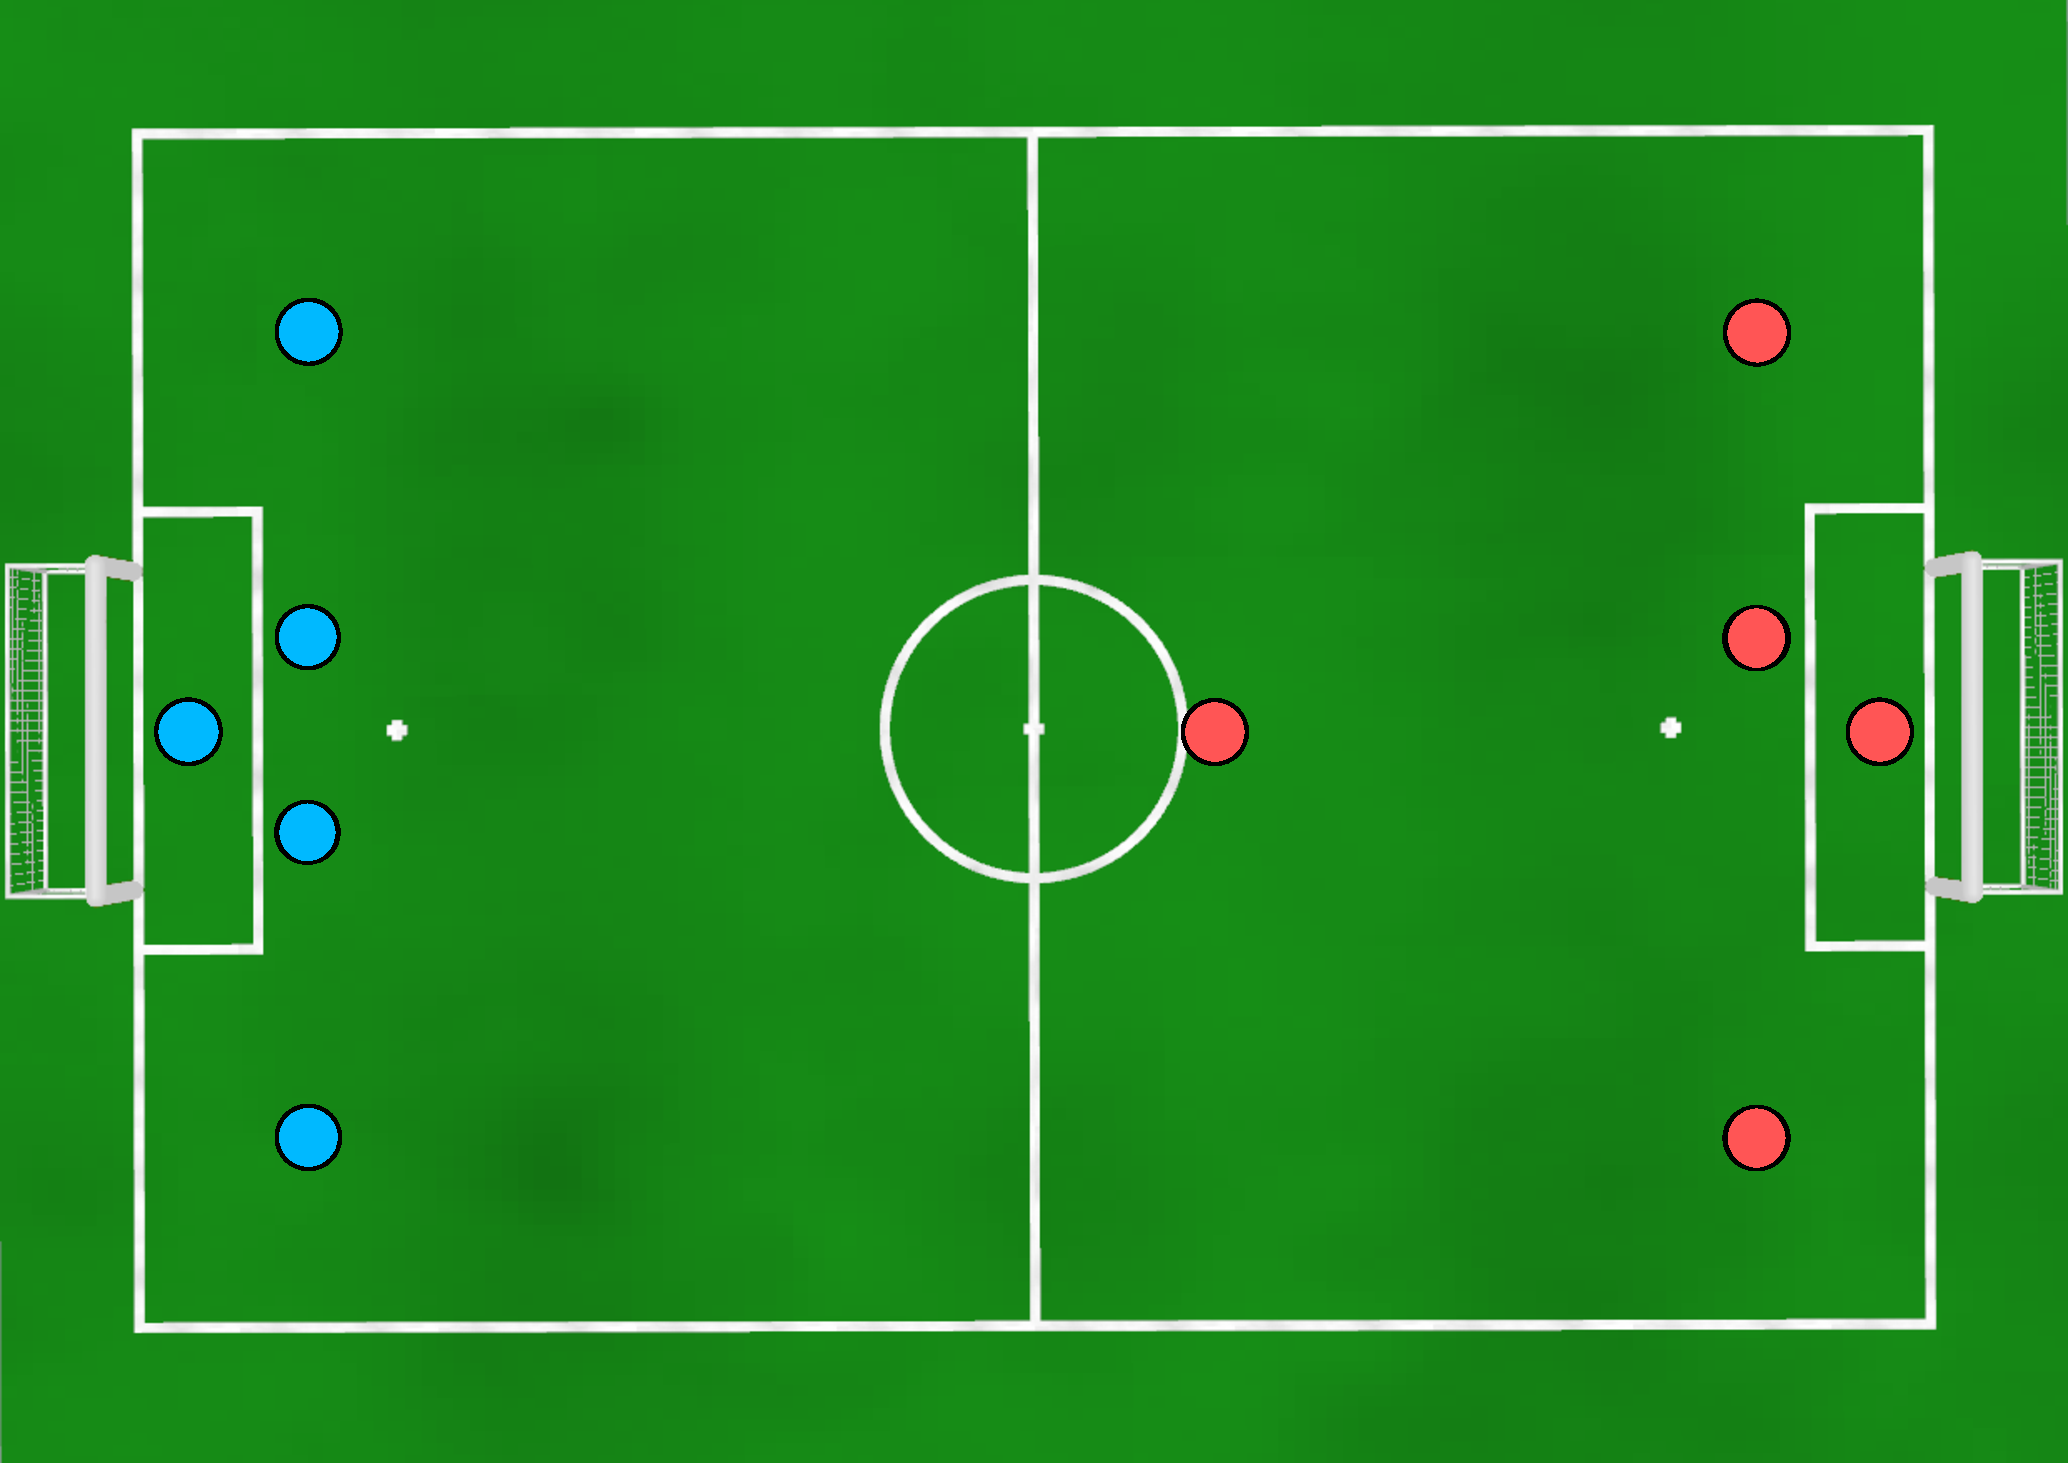
\includegraphics[width=\columnwidth]{figs/manual-placement-cs.pdf}}
\caption{Challenge Shield manual setup for kick-off.  The attacking team is on the right.}
\label{fig:ko-manual}
\end{figure}

\subsubsection{Kick-In (Section \ref{sec:kick_in})}
\label{sub:cc-kick-in}

The position the ball is placed for a kick-in is modified as follows:
\begin{itemize}
    \item If the ball goes over a sideline, the ball is placed approximately 2-ball-widths in from the sideline perpendicular to the point where the ball went out.
    \item If the ball goes over a sideline, closer to an end-line than the corresponding penalty spot, the ball is placed 2-ball-widths in from the sideline and in-line with the penalty spot.
    \item For a corner kick, the ball is also placed 2-ball-widths in from the sideline and in-line with the penalty spot.
\end{itemize}

\subsubsection{Free-Kick Procedure (Section \ref{sec:free_kick})}
\label{sub:cc-free-kick-procedure}

The procedure for a \emph{Free Kick} is replaced with a procedure similar to the Penalty Free Kick.

When a Free Kick is initiated the head referee will announce a Free Kick, calling one of:
\begin{enumerate}
  \item For a \textit{Pushing Free Kick}: ``Foul \textless color\textgreater \textless number\textgreater'' for the pushing robot.
  \item For all other free kicks: ``Kick-in/Goal Kick/Corner Kick \textless team\textgreater'' for the team that did not last touch the ball.
\end{enumerate}

The GameController will then activate the substate for the respective free kick. Note that in the case of the Pushing Free Kick the substate is activated automatically through the ``Foul''.
The game changes to the \textit{Ready} state.
This denotes that the robot's are given time to setup and prepare for the free kick.
The game clock is \textit{paused} during finals games only.

The head referees \emph{immediately} places the ball on the spot for the Free Kick.
Players have \qty{\SCFreeKickSetupTime}{\second} to get into position for the Free Kick.
At the end of \qty{\SCFreeKickSetupTime}{\second}, the game changes to the \textit{Set} state.
Similar to a kick-off, during the Set state the robots are waiting for the Free Kick to commence.
Standard penalties apply.
Additionally, no player may touch the ball and defending players may not be within \FreeKickRadius of the ball.
Defensive players that violate this restrictions are penalised with the ``Illegal Positioning'' penalty (see Section~\ref{sec:illegal_positioning}) which results in a standard removal penalty~(see Section~\ref{sec:removal_penalty}).

During Set, the team leader of the attacking team may call ``Manual Free Kick Placement''.
If this is called, the referee should move the attacking robot that is closest to the ball, to be placed \SCFreeKickDistance behind the ball, on a line between the ball and the centre of the goal.

The referee signals the Free Kick commences by blowing the whistle once, and calling ``Playing''.
The game switches to the \textit{free kick} sub-state of the \textit{Playing} game state, and the game clock is resumed.
Note that the GameContoller signal is \emph{not} delayed for this procedure in the Challenge Shield.
The attacking team has \qty{\SCFreeKickTime}{\second} to complete the Free Kick.
During the Free Kick, all players may move freely, however, defensive robots may not enter within \FreeKickRadius of the ball Defensive players that violate this restrictions are penalised with the ``Illegal Positioning'' penalty (see Section~\ref{sec:illegal_positioning}).
Note that in all Free Kicks the Indirect Kick rule applies.

The head referee will announce a Free Kick is completed, by ``Ball Free'', and the GameController resumes the game state \emph{playing}. Note that the substate will be automatically left after the \qty{\SCFreeKickTime}{\second} time period expires.

\subsubsection{Free-Kick: Penalty Kick (Section \ref{sec:free_kick})}
\label{sub:cc-fk-penalty-kick}

The \emph{Penalty Kick} rule (and associated procedure) is removed, and replaced by a \emph{Pushing Free Kick}.

The ball is still placed on the penalty spot for a \emph{Pushing Free Kick} awarded against the defending team within their own penalty box for the \emph{Pushing Free Kick}.

\subsubsection{Penalty Kick Procedure (Section \ref{sec:penalty_free_kick})}
\label{sub:cc-penalty-kick-procedure}

Removed for the Challenge Shield, and replaced by a standard \emph{Pushing Free Kick}.

\subsubsection{Request for Pickup (Section \ref{sec:request_for_pickup})}
\label{sub:cc-request-for-pickup}

During the \emph{Ready} and \emph{Playing} states, a team may call a request for pick-up for \textbf{software related failures}, provided that:
\begin{itemize}
    \item The player is at least \qty{1}{\meter} away from the ball.
    \item The head referee determines that team requesting pickup would not gain an advantage by removing the robot.
\end{itemize}

Note that, during the \emph{Set} state of a \emph{Free Kick} under the Challenge Shield procedure, a team may call a request for pick-up on any robot for any reason.

\subsubsection{Standard Removal Penalty (Section \ref{sec:removal_penalty})}
\label{sub:cc-standard-removal-penalty}

The duration of the standard-removal-penalty-time is reduced to \qty{\CSStandardPenaltyTime}{\second}.

The penalty time \emph{does not} increase each time a team commits an infraction so that all penalties result in a fixed duration of \qty{\CSStandardPenaltyTime}{\second}.

\subsection{Referee Selection and Requirements}
\label{sec:refSelection}
During pool play, the games will be refereed by members of teams from a different pool.

Each team has to referee a number of games. A schedule will be released specifying the games for which each team is required to provide two referees. Referees should report to the appropriate field at least five minutes before the game is scheduled to start.

If a team fails to provide two referees for a game in which they are scheduled to provide referees, it will be noted by the organizing committee and recorded as a \textbf{qualification penalty} (\cref{sec:qualificationPenalties}).

For each of the games, a team will be required either to provide the head referee and the operator of the GameController, or the two assistant referees.  The two teams assigned to referee a game shall decide among themselves which roles each team will fulfill. Note, however, that the head referee and the GameController should always be from the same team.

A team may swap their scheduled refereeing duties with another team, but the team listed on the referee schedule will be held accountable if referees fail to appear for a game they are scheduled to referee.

The requirement to referee may be an extreme hardship for extremely small teams.  If a team believes providing two referees for games will be an extreme hardship, they must send an email explaining their situation to the Organizing Committee and Technical Committee at least two weeks before the first set up day of the competition.  The Organizing and Technical Committees will then consider the request and attempt to find an acceptable solution.

Referees must have good knowledge of the rules as applied in the tournament, and the operator of the GameController must be experienced in using that software. Referees and the GameController should be selected among the more senior members of a team, and preferably have prior experience with games in the RoboCup Standard Platform league.

In each game, each of the teams playing shall be able to veto one and only one eligible referee with no reason required. The veto must be delivered before the start of the ready phase or during a stoppage of play.


\subsection{Subsequent Year Pre-Qualification Procedure}
\label{sec:preQual}
Up to 11 teams may become pre-qualified for the subsequent year's team competition by fulfilling one of the following criteria:
\begin{itemize}
    \item Reaching the quarter-finals of the Champions Cup
    \item Reaching the final of the Challenge Shield
    \item Being the team with the best overall result in the technical challenges that is not pre-qualified by other means, and finishing at worst 5th in the technical challenges.
\end{itemize}

However, pre-qualified teams must do all the following in order to remain pre-qualified:
\begin{itemize}
\item Post in a publicly available location a team research report describing their work for the 2019 competition
\item Publicly release code from that year's codebase, either in the form of a complete release (perhaps without behavior) or limited libraries.  This release must be documented and coded in a way where it can be used by others.
\item Submit a shortened application as required by the call for participation for the subsequent year's competition.
\end{itemize}

\subsection{Qualification Penalties}
\label{sec:qualificationPenalties}

There are a number of offenses which lead to qualification penalties being recorded against a team. These are as follows:
\begin{itemize}
    \item Withdrawing from RoboCup after the final commitment deadline
    \item Failing to referee when assigned (\cref{sec:refSelection})
    \item Forfeiting a game (\cref{sec:forfeit})
\end{itemize}

A team cannot be pre-qualified for RoboCup in the year following a qualification penalty. Furthermore, a qualification penalty is considered by the Technical Committee when reviewing applications and will negatively affect the assessment of a team's application. Multiple penalties accumulate and will result in an even more negative assessment of a team's application. Qualification penalties are considered for a period of three years following the offense.

Whenever a qualification penalty is recorded, all relevant details including any possible mitigating circumstances are also recorded and these will also inform the assessment of a team's application.

\subsection{Disqualification during Competition}
\label{sec:disqualification_during_comp}

A team may be disqualified during the RoboCup competition for:
\begin{itemize}
  \item A serious violation of the terms of a team's qualification
  \item Gaining a Qualification Penalty during the course of the competition~(\cf \cref{sec:qualificationPenalties})
  \item A serious breach of ethics, or serious behavior unbecoming of participants of RoboCup.
\end{itemize}

\textbf{Example.} A team promises to use their novel contribution in RoboCup games, but fails to do so.
Alternatively, a team deliberately misleads the technical committee about the novelty of their work and/or their contribution to the league, such that they are deemed to have copied another team.

A team can \textit{only} be disqualified by a decision of the \textit{Board of Trustees of the RoboCup Federation}.
The RoboCup Soccer SPL executive must petition the board in writing at their soonest possible availability.
The executive must simultaneously inform the relevant team of the petition in writing.

A disqualified team automatically forfeits all games~(\cf \cref{sec:forfeit}).
For practicality, the disqualification should not apply \textit{retroactively}.
However, by majority vote of the team leaders, provisions for retroactive disqualification may be made in the fairness of the affected teams.
